%%%%%%%%%%%%%%%%%%%%%%%%%%%%%%%%%%%%%%%%%
% Beamer Presentation
% LaTeX Template
% Version 1.0 (10/11/12)
%
% This template has been downloaded from:
% http://www.LaTeXTemplates.com
%
% License:
% CC BY-NC-SA 3.0 (http://creativecommons.org/licenses/by-nc-sa/3.0/)
%
%%%%%%%%%%%%%%%%%%%%%%%%%%%%%%%%%%%%%%%%%

%----------------------------------------------------------------------------------------
%	PACKAGES AND THEMES
%----------------------------------------------------------------------------------------

%\documentclass{beamer}
%\usepackage{enumitem}
%\usepackage{booktabs}  
\documentclass{beamer} 
\usetheme{metropolis}
\usepackage{algorithmicx}
\usepackage[latin1]{inputenc}
\usefonttheme{professionalfonts}
\usepackage{times}
\usepackage{tikz}
\usepackage{amsmath}
\usepackage{fancyvrb}
\usepackage{listings}
\usepackage{graphicx}
\graphicspath{{./img/}}
%\usepackage{algorithm,algorithmic}
\usetikzlibrary{arrows,shapes}   
%\renewcommand{\algorithmicrequire}{\textbf{Input:}}
%\renewcommand{\algorithmicensure}{\textbf{Output:}}
\def \S {\mathbf{S}}
\def \A {\mathcal{A}}
\def \X {\mathcal{X}}
\def \Ab {\bar{\A}}
\def \R {\mathbb{R}}
\def \Kt {\widetilde{K}}
\def \k {\mathbf{k}}
\def \w {\mathbf{w}}
\def \v {\mathbf{v}}
\def \t {\mathbf{t}}
\def \x {\mathbf{x}}
\def \Se {\mathcal{S}}
\def \E {\mathrm{E}}
\def \Rh {\widehat{R}}
\def \x {\mathbf{x}}
\def \p {\mathbf{p}}
\def \a {\mathbf{a}}
\def \diag {\mbox{diag}}
\def \b {\mathbf{b}}
\def \e {\mathbf{e}}
\def \ba {\boldsymbol{\alpha}}
\def \c {\mathbf{c}}
\def \tr {\mbox{tr}}
\def \d {\mathbf{d}}
\def \z {\mathbf{z}}
\def \s {\mathbf{s}}
\def \bh {\widehat{b}}
\def \y {\mathbf{y}}
\def \u {\mathbf{u}}
%\def \L {\mathcal{L}}
\def \H {\mathcal{H}}
\def \g {\mathbf{g}}
\def \F {\mathcal{F}}
\def \I {\mathbb{I}}
\def \P {\mathcal{P}}
\def \Q {\mathcal{Q}}
\def \xh {\widehat{\x}}
\def \wh {\widehat{\w}}
\def \ah {\widehat{\alpha}}
\def \Rc {\mathcal R}

\def \Bh {\widehat B}
\def \Ah {\widehat A}
\def \Uh {\widehat U}
\def \Ut {\widetilde U}
\def \B {\mathbf B}
\def \C {\mathbf C}
\def \U {\mathbf U}
\def \Kh {\widehat K}
\def \fh {\widehat f}
\def \yh {\widehat y}
\def \Xh {\widehat{X}}
\def \Fh {\widehat{F}}


\def \y {\mathbf{y}}
\def \E {\mathrm{E}}
\def \x {\mathbf{x}}
\def \g {\mathbf{g}}
\def \D {\mathcal{D}}
\def \z {\mathbf{z}}
\def \u {\mathbf{u}}
\def \H {\mathcal{H}}
\def \Pc {\mathcal{P}}
\def \w {\mathbf{w}}
\def \r {\mathbf{r}}
\def \R {\mathbb{R}}
\def \S {\mathcal{S}}
\def \regret {\mbox{regret}}
\def \Uh {\widehat{U}}
\def \Q {\mathcal{Q}}
\def \W {\mathcal{W}}
\def \N {\mathcal{N}}
\def \A {\mathcal{A}}
\def \q {\mathbf{q}}
\def \v {\mathbf{v}}
\def \M {\mathcal{M}}
\def \c {\mathbf{c}}
\def \ph {\widehat{p}}
\def \d {\mathbf{d}}
\def \p {\mathbf{p}}
\def \q {\mathbf{q}}
\def \db {\bar{\d}}
\def \dbb {\bar{d}}
\def \I {\mathcal{I}}
\def \xt {\widetilde{\x}}
\def \f {\mathbf{f}}
\def \a {\mathbf{a}}
\def \b {\mathbf{b}}
\def \ft {\widetilde{\f}}
\def \bt {\widetilde{\b}}
\def \h {\mathbf{h}}
\def \B {\mathbf{B}}
\def \bts {\widetilde{b}}
\def \fts {\widetilde{f}}
\def \Gh {\widehat{G}}
\def \G {\mathcal {G}}
\def \bh {\widehat{b}}
\def \fh {\widehat{f}}
\def \wh {\widehat{\w}}
\def \vb {\bar{v}}
\def \zt {\widetilde{\z}}
\def \zts {\widetilde{z}}
\def \s {\mathbf{s}}
\def \gh {\widehat{\g}}
\def \vh {\widehat{\v}}
\def \Sh {\widehat{S}}
\def \rhoh {\widehat{\rho}}
\def \hh {\widehat{\h}}
\def \C {\mathcal{C}}
\def \V {\mathcal{L}}
\def \t {\mathbf{t}}
\def \xh {\widehat{\x}}
\def \Ut {\widetilde{U}}
\def \wt {\widetilde{\w}}
\def \Th {\widehat{T}}
\def \Ot {\tilde{\mathcal{O}}}
\def \X {\mathcal{X}}
\def \nb {\widehat{\nabla}}
\def \K {\mathcal{K}}
\def \P {\mathbb{P}}
\def \T {\mathcal{T}}
\def \F {\mathcal{F}}
\def \ft{\widetilde{f}}
\def \xt {\widetilde{x}}
\def \Rt {\mathcal{R}}
\def \Rb {\bar{\Rt}}
\def \wb {\bar{\w}}
%\mode<presentation> {
	
	% The Beamer class comes with a number of default slide themes
	% which change the colors and layouts of slides. Below this is a list
	% of all the themes, uncomment each in turn to see what they look like.
	
	%\usetheme{default}
	%\usetheme{AnnArbor}
	%\usetheme{Antibes}
	%\usetheme{Bergen}
	%\usetheme{Berkeley}
	%\usetheme{Berlin}
	%\usetheme{Boadilla}
	%\usetheme{CambridgeUS}
	%\usetheme{Copenhagen}
	%\usetheme{Darmstadt}
	%\usetheme{Dresden}
	%\usetheme{Frankfurt}
	%\usetheme{Goettingen}
	%\usetheme{Hannover}
	%\usetheme{Ilmenau}
	%\usetheme{JuanLesPins}
	%\usetheme{Luebeck}
	%\usetheme{Madrid}
	%\usetheme{Malmoe}
	%\usetheme{Marburg}
	%\usetheme{Montpellier}
	%\usetheme{PaloAlto}
	%\usetheme{Pittsburgh}
	%\usetheme{Rochester}
	%\usetheme{Singapore}
	%\usetheme{Szeged}
	%\usetheme{Warsaw}
	
	% As well as themes, the Beamer class has a number of color themes
	% for any slide theme. Uncomment each of these in turn to see how it
	% changes the colors of your current slide theme.
	
	%\usecolortheme{albatross}
	%\usecolortheme{beaver}
	%\usecolortheme{beetle}
	%\usecolortheme{crane}
	%\usecolortheme{dolphin}
	%\usecolortheme{dove}
	%\usecolortheme{fly}
	%\usecolortheme{lily}
	%\usecolortheme{orchid}
	%\usecolortheme{rose}
	%\usecolortheme{seagull}
	%\usecolortheme{seahorse}
	%\usecolortheme{whale}
	%\usecolortheme{wolverine}
	
	%\setbeamertemplate{footline} % To remove the footer line in all slides uncomment this line
	%\setbeamertemplate{footline}[page number] % To replace the footer line in all slides with a simple slide count uncomment this line
	
	%\setbeamertemplate{navigation symbols}{} % To remove the navigation symbols from the bottom of all slides uncomment this line
%}

\usepackage{graphicx} % Allows including images
\usepackage{booktabs} % Allows the use of \toprule, \midrule and \bottomrule in tables

%----------------------------------------------------------------------------------------
%	TITLE PAGE
%----------------------------------------------------------------------------------------

\title{Efficient Distributed Stochastic Dual Coordinate Ascent} % The short title appears at the bottom of every slide, the full title is only on the title page

%\author{John Smith} % Your name
\author{Jeff Hajewski \\ Mingrui Liu}
\date{May 3, 2017}
\institute{University of Iowa}

%\date{\today} % Date, can be changed to a custom date
\AtBeginSubsection[]
{
	\begin{frame}<beamer>{Outline}
		\tableofcontents[currentsection,currentsubsection]
	\end{frame}
}
\begin{document}
	
	\begin{frame}
		\titlepage % Print the title page as the first slide
	\end{frame}
	
	%\begin{frame}
	%	\frametitle{Overview} % Table of contents slide, comment this block out to remove it
	%	\tableofcontents % Throughout your presentation, if you choose to use \section{} and \subsection{} commands, these will automatically be printed on this slide as an overview of your presentation
	%\end{frame}
	\begin{frame}{Outline}
		\tableofcontents
	\end{frame}
	%----------------------------------------------------------------------------------------
	%	PRESENTATION SLIDES
	%----------------------------------------------------------------------------------------
	
	%------------------------------------------------
\section{Problem Overview}

\begin{frame}{Problem Overview - The Primal Problem}
	Many machine learning problems can be formulated as the Regularized Finite Sum Minimization (RFSM) problem.
  \vspace{1em}
	\begin{equation}
		\label{RLM}
		\min_{w\in\R^d}P(w)
	\end{equation}
  \vspace{1.5em}\\
  where 
  \begin{align*}
    P(w) &= \frac{1}{n}\sum_{i=1}^{n}\phi(w^\top x_i,y_i)+\lambda g(w)\\
    w, x_i & \in \R^d, \text{ for } i = 1, \dots, n\\
    y_i & \in \R, \text{ for } i = 1, \dots, n\\
    \phi(z,y) & \text{ is convex in $z$}\\
    g(w) & \text{ is convex in $w$}\\
  \end{align*}
  
\end{frame}

\begin{frame}{Problem Overview - The Dual Problem}
  We consider the case when $g(w)=\frac{1}{2}\|w\|_2^2$, then the dual problem is given by
  \vspace{1em}
  \begin{equation}
    \max_{\alpha \in \R^n} D(\alpha)
  \end{equation}
  where 
  \begin{align*}
    D(\alpha) &= \frac{1}{n}\sum_{i=1}^n -\phi^*_i(-\alpha_i) -
    \frac{\lambda}{2}\Big|\Big|\frac{1}{\lambda n}\sum_{i=1}^n\alpha_i x_i\Big|\Big|^2\\
    x_i & \in \R^d, \text{ for } i = 1, \dots, n\\
    \alpha & \in \R^n\\
    \phi^*_i(u) &= \max_z (zu - \phi_i(z))
  \end{align*}
\end{frame}
%
%\subsection{Related Work}
\begin{frame}{Related Work}
  The two key papers influencing our work are:
	\begin{itemize}
	  \item  Stochastic Dual Coordinate Ascent (SDCA) \cite{shalev2013stochastic}
	  \item Distributed SDCA  \cite{yang2013trading,yang2013analysis}
	\end{itemize}
\end{frame}
	%----------------------------------------------------------------------------------------

\begin{frame}{What is SDCA?}
  \begin{itemize}
    \item \textbf{SDCA} - randomly pick a coordinate axis of $\mathbf{\alpha}
      \in \R^n$, find update that best improves
      the objective\vspace{1em}
    \item \textbf{Distributed SDCA} - randomly pick $k$ coordinate axes of
      $\mathbf{\alpha} \in \R^n$, simultaneously
      find updates that best improve the objective (independently)
  \end{itemize}
\end{frame}
\begin{frame}{SDCA Algorithm}
	SDCA procedure:
	\begin{itemize}
		\item Let $w^{(0)}=w(\alpha^{(0)})$
		\item \textbf{Iterate}: for $t=1,2,\ldots,T$
		\begin{itemize}
			\item Randomly pick $i$
			\item \textcolor{red}{Find $\triangle\alpha_i$ to maximize $-\phi_i^*(-(\alpha^{(t-1)}+\triangle\alpha_i))-\frac{\lambda n}{2}\|w^{(t-1)}+(\lambda n)^{-1}\triangle \alpha_i x_i\|^2$}
			\item \textcolor{red}{$\alpha^{(t)}\leftarrow\alpha^{(t-1)}+\triangle\alpha_ie_i$}
			\item \textcolor{red}{$w^{(t)}\leftarrow w^{(t-1)}+(\lambda n)^{-1}\triangle\alpha_i x_i$}
		\end{itemize}
	\item Output (Random option):\\
			Let $\bar{\alpha}=\alpha^{(t)}$ and $\bar{w}=w^{(t)}$ for some random $t\in T_0+1,\ldots,T$\\
	\textbf{Return} $\bar{w}$
	\end{itemize}
	\textbf{Remark:} The red steps spend the largest proportion of computing resources. 
\end{frame}

\begin{frame}[standout]
  What if we ran SDCA on the GPU?
\end{frame}

\begin{frame}{Parallelizing SDCA}
  Two approaches:
	\begin{itemize}
    \item Naive approach: simply parallelize all tensor operations (e.g., dot
      product, matrix-vector multiplication, etc.) \pause
  \item Better: mimic the distributed apporach by \cite{yang2013trading} on a GPU
	\end{itemize}
\end{frame}
\section{Implementation}
\begin{frame}{Main Points}
  The key area of concern:
  \begin{itemize}
    \item Memory
      \begin{itemize}
        \item Allocation \pause
        \item Communication (via PCIE bus rather than network) \pause
        \item How can we reduce cognitive load of writing this code?
      \end{itemize}
  \end{itemize}
\end{frame}

\begin{frame}{Dealing with Memory Allocation}
  Naive approach:
  \VerbatimInput[fontsize=\small]{allocExample.txt}
  On a small dataset(200 points in $\mathbb{R}^3$) we hit over 200k allocations,
  which comprised nearly \textbf{95\%} of the GPU compute time ($\approx 13$
    seconds).
\end{frame}

\begin{frame}[standout]
  Can we do better?\\ \pause
  Yes!
\end{frame}


\begin{frame}{Dealing with Memory Allocation}
  Better approach:
  \VerbatimInput[fontsize=\small]{allocImproved.txt}
  The use of static class pointers reduced the 200k allocations down to only
  \textbf{3 memory allocations}, which comprised only \textbf{0.03\%} compute
    time ($\approx 180 \mu s$).
\end{frame}

\begin{frame}[standout]
  What about the cost of communication?
\end{frame}

\begin{frame}{Communication Costs}
  Copying data to and from the GPU is the next most expensive operation.
  \begin{itemize}
    \item About 50\% of the compute time, or 768 ms (using the same toy dataset,
      after we have fixed the memory allocation issue) \pause
    \item Mostly unnecessary!
  \end{itemize}
\end{frame}

\begin{frame}{Communication Costs}
  Consider the following algorithm using the GPU:
  \begin{algorithmic}[1]
    \State $\Delta \omega_i \gets f(\mathbf{x}, \omega)$
    \State $\omega_i \gets \omega_i + \Delta \omega_i$
  \end{algorithmic}
  
  To handle this efficiently we should:
  \begin{itemize}
      \pause
    \item Reuse $\omega$ in step 2 since we already moved it to the GPU for step
      1 \pause
    \item Perform step 2 on the GPU since the data is already there. No need to
      pull it off and then move it back to the GPU
  \end{itemize}
\end{frame}

\begin{frame}{Communication Costs}
  The sad reality is this is quite complicated.

  \begin{itemize}
    \item Lots of book-keeping
    \item Are there edge cases?
    \item Need to watch out for memory leaks. Remember, \textbf{no} GC!
  \end{itemize}
\end{frame}

\begin{frame}[standout]
  How can we handle this complexity?
\end{frame}

\begin{frame}{Wrappers}
  We use wrappers (also known as decorators) to add additional functionality to
  our code. For example,
  \VerbatimInput[fontsize=\small]{wrapperEx.txt}
\end{frame}

\begin{frame}{Wrappers}
  To handle the flow of data from GPU to CPU, as well as book-keeping, we can
  use something like this:
  \VerbatimInput[fontsize=\small]{dataEx.txt}
\end{frame}

\begin{frame}[standout]
  What about results?
\end{frame}

\begin{frame}{Distributed SDCA}
  \begin{itemize}
    \item We have a closed-form solution for $\Delta \alpha$ \pause
    \item The computationally intensive task is $\omega^\top x_i$ \pause
    \item This means for $k$ coordinate axes, we want to compute $X\omega$,
      where $X = (x_{i_1}^\top x_{i_2}^\top \cdots x_{i_k}^\top)^\top$. \pause
  \end{itemize}
  We can reformulate the distributed version as matrix-vector multiplication.
  This is just an extension of the naive approach!
\end{frame}

\begin{frame}{Distributed SDCA - The Challenge}
  So what is the challenge?\\ \pause
  Our memory management class is poorly written
  \begin{itemize}
    \item $X$ is a matrix now, not a vector\pause
    \item However, we have only allocated memory for vectors
  \end{itemize}
\end{frame}

\begin{frame}{Results - Challenges}
  We are still finalizing results. There is a lot of non-trivial structural code
  behind this.
  \begin{itemize}
    \item Loading data \pause
    \item CUDA can be challenging  - communication is slowing us down\pause
    \item Algorithm \pause
    \item Algorithm performance tracking \pause
    \item Expect distributed SDCA to be the fastest, followed by CUDA
      accelerated SDCA, followed by SDCA
  \end{itemize}
\end{frame}

\begin{frame}{Results - Australian Dataset ($\R^{14}$, 690 points)}
  Naive approach\\
  \begin{figure}
    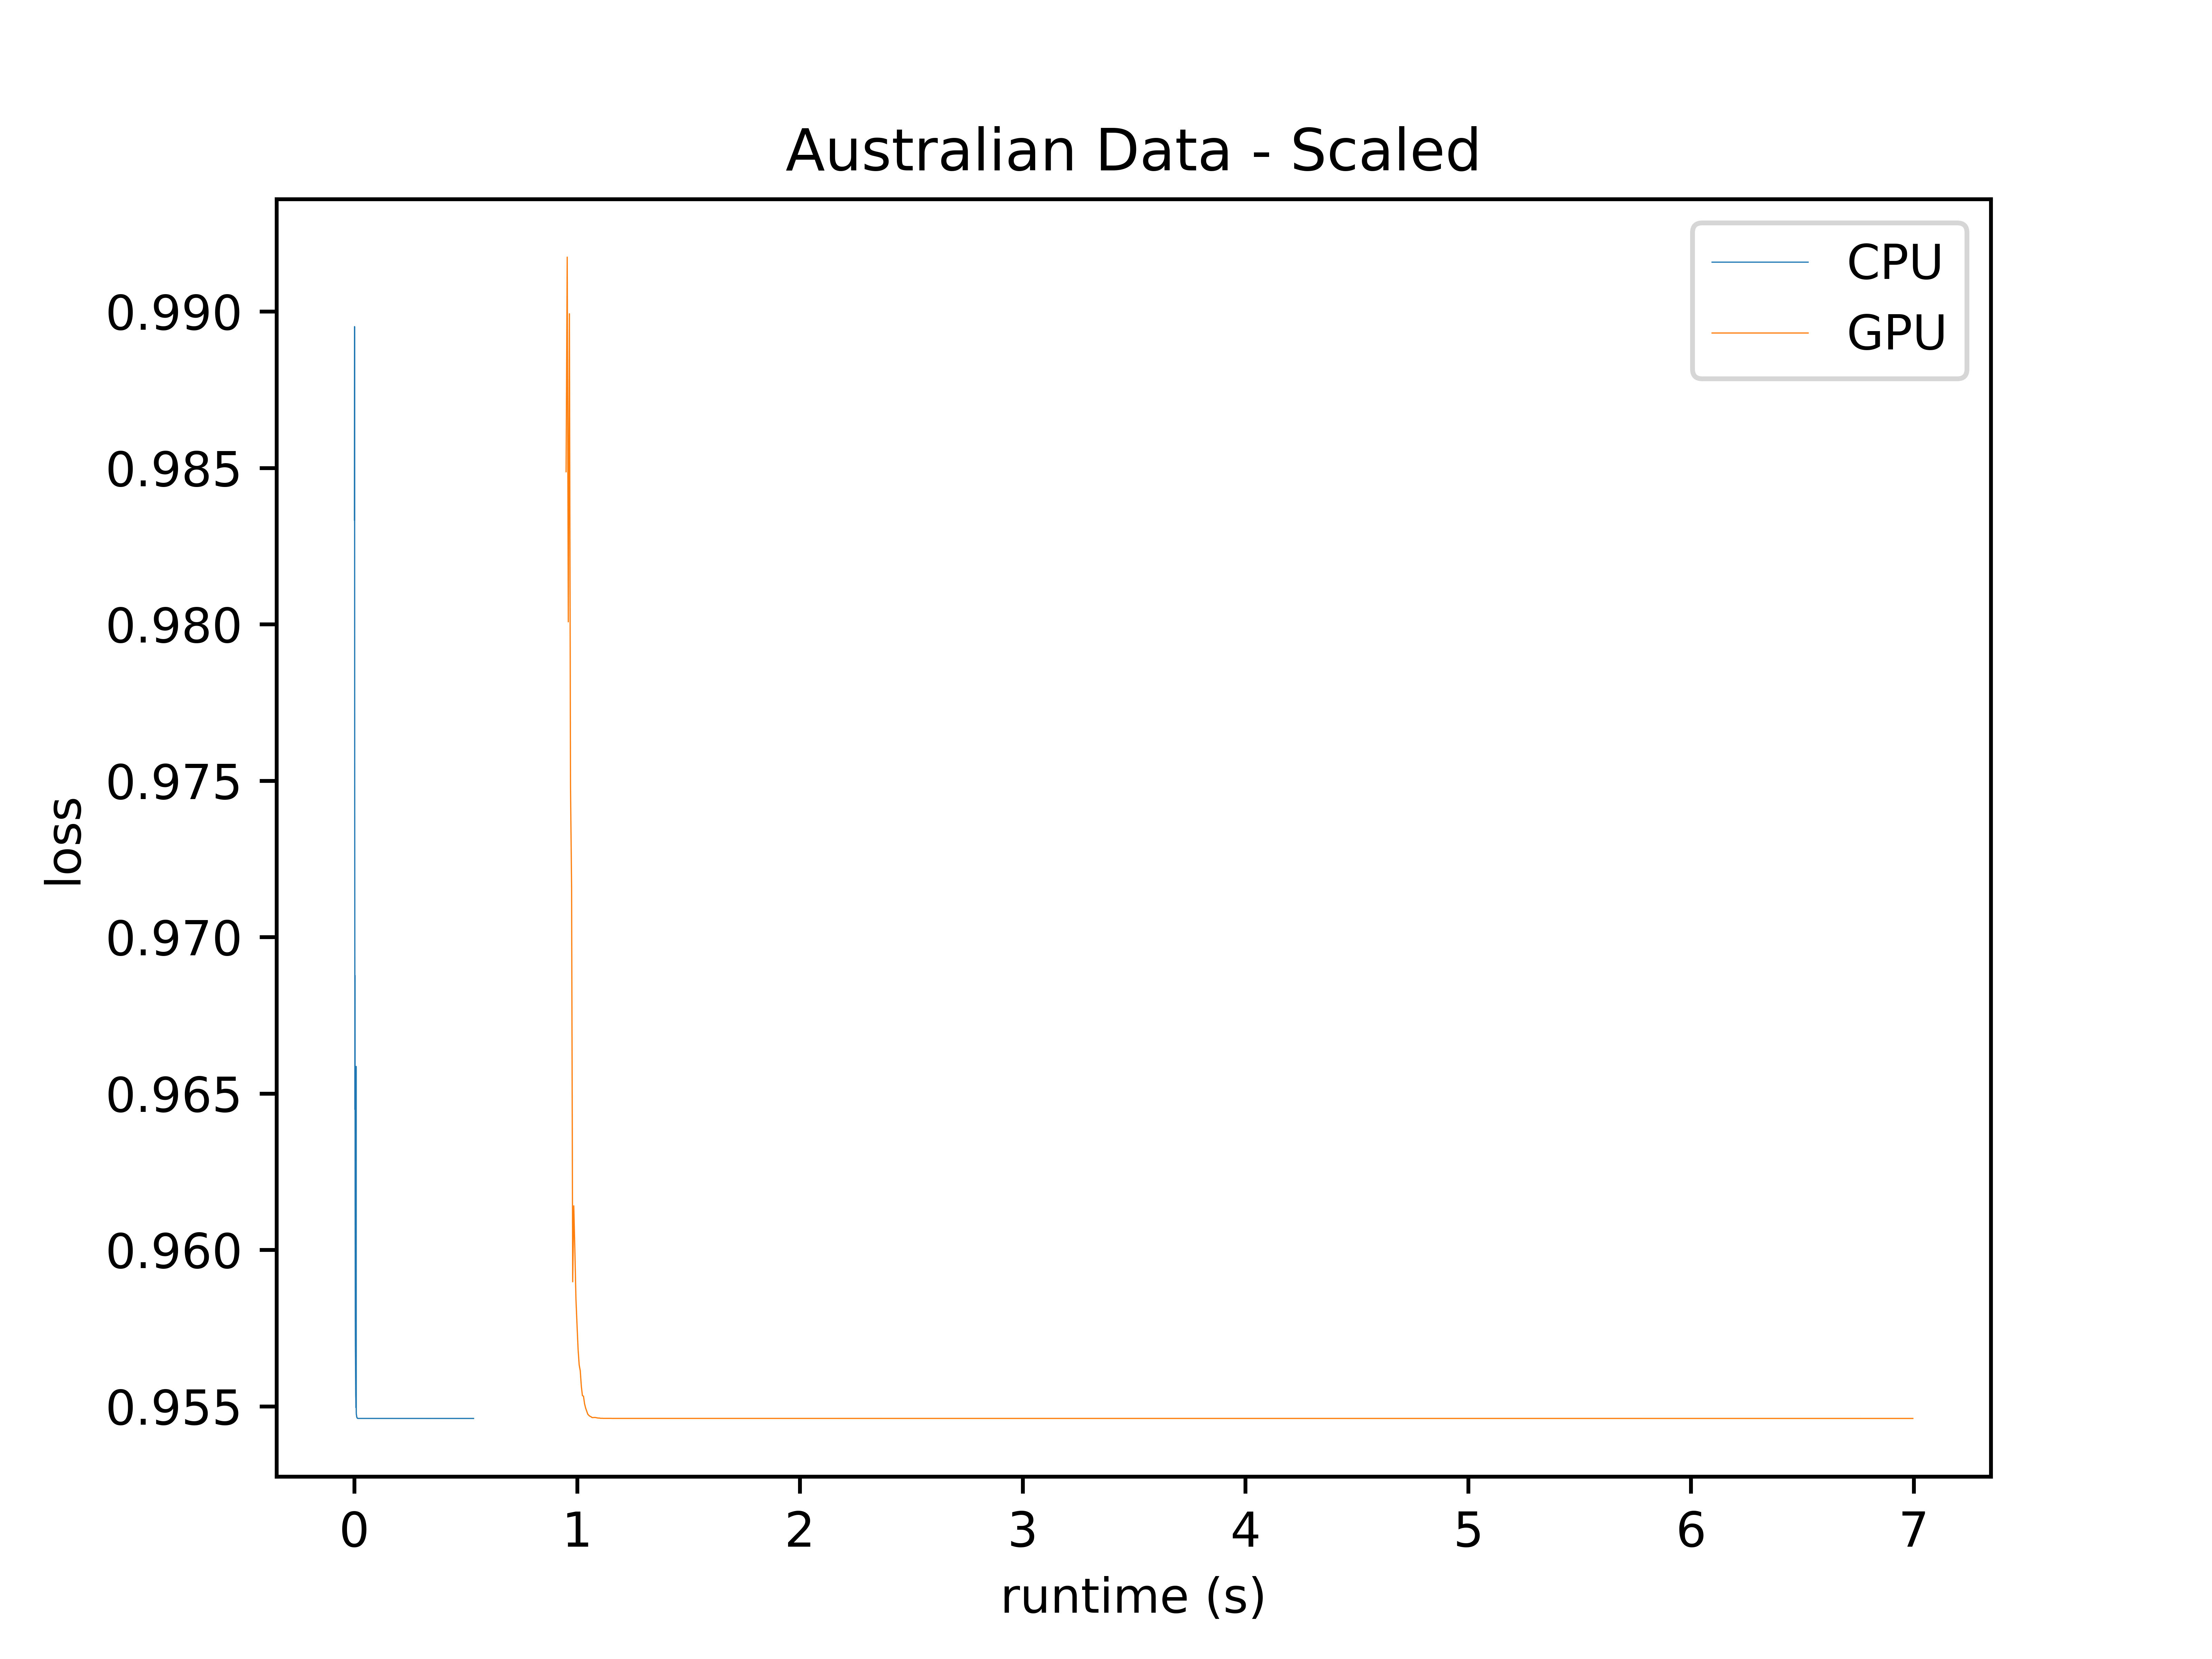
\includegraphics[scale=0.5]{cpu_vs_gpu}
\end{figure}
\end{frame}

\begin{frame}{Results - Generated Dataset ($\R^{10k}$, 1000 points)}
  Naive approach\\
  \begin{figure}
    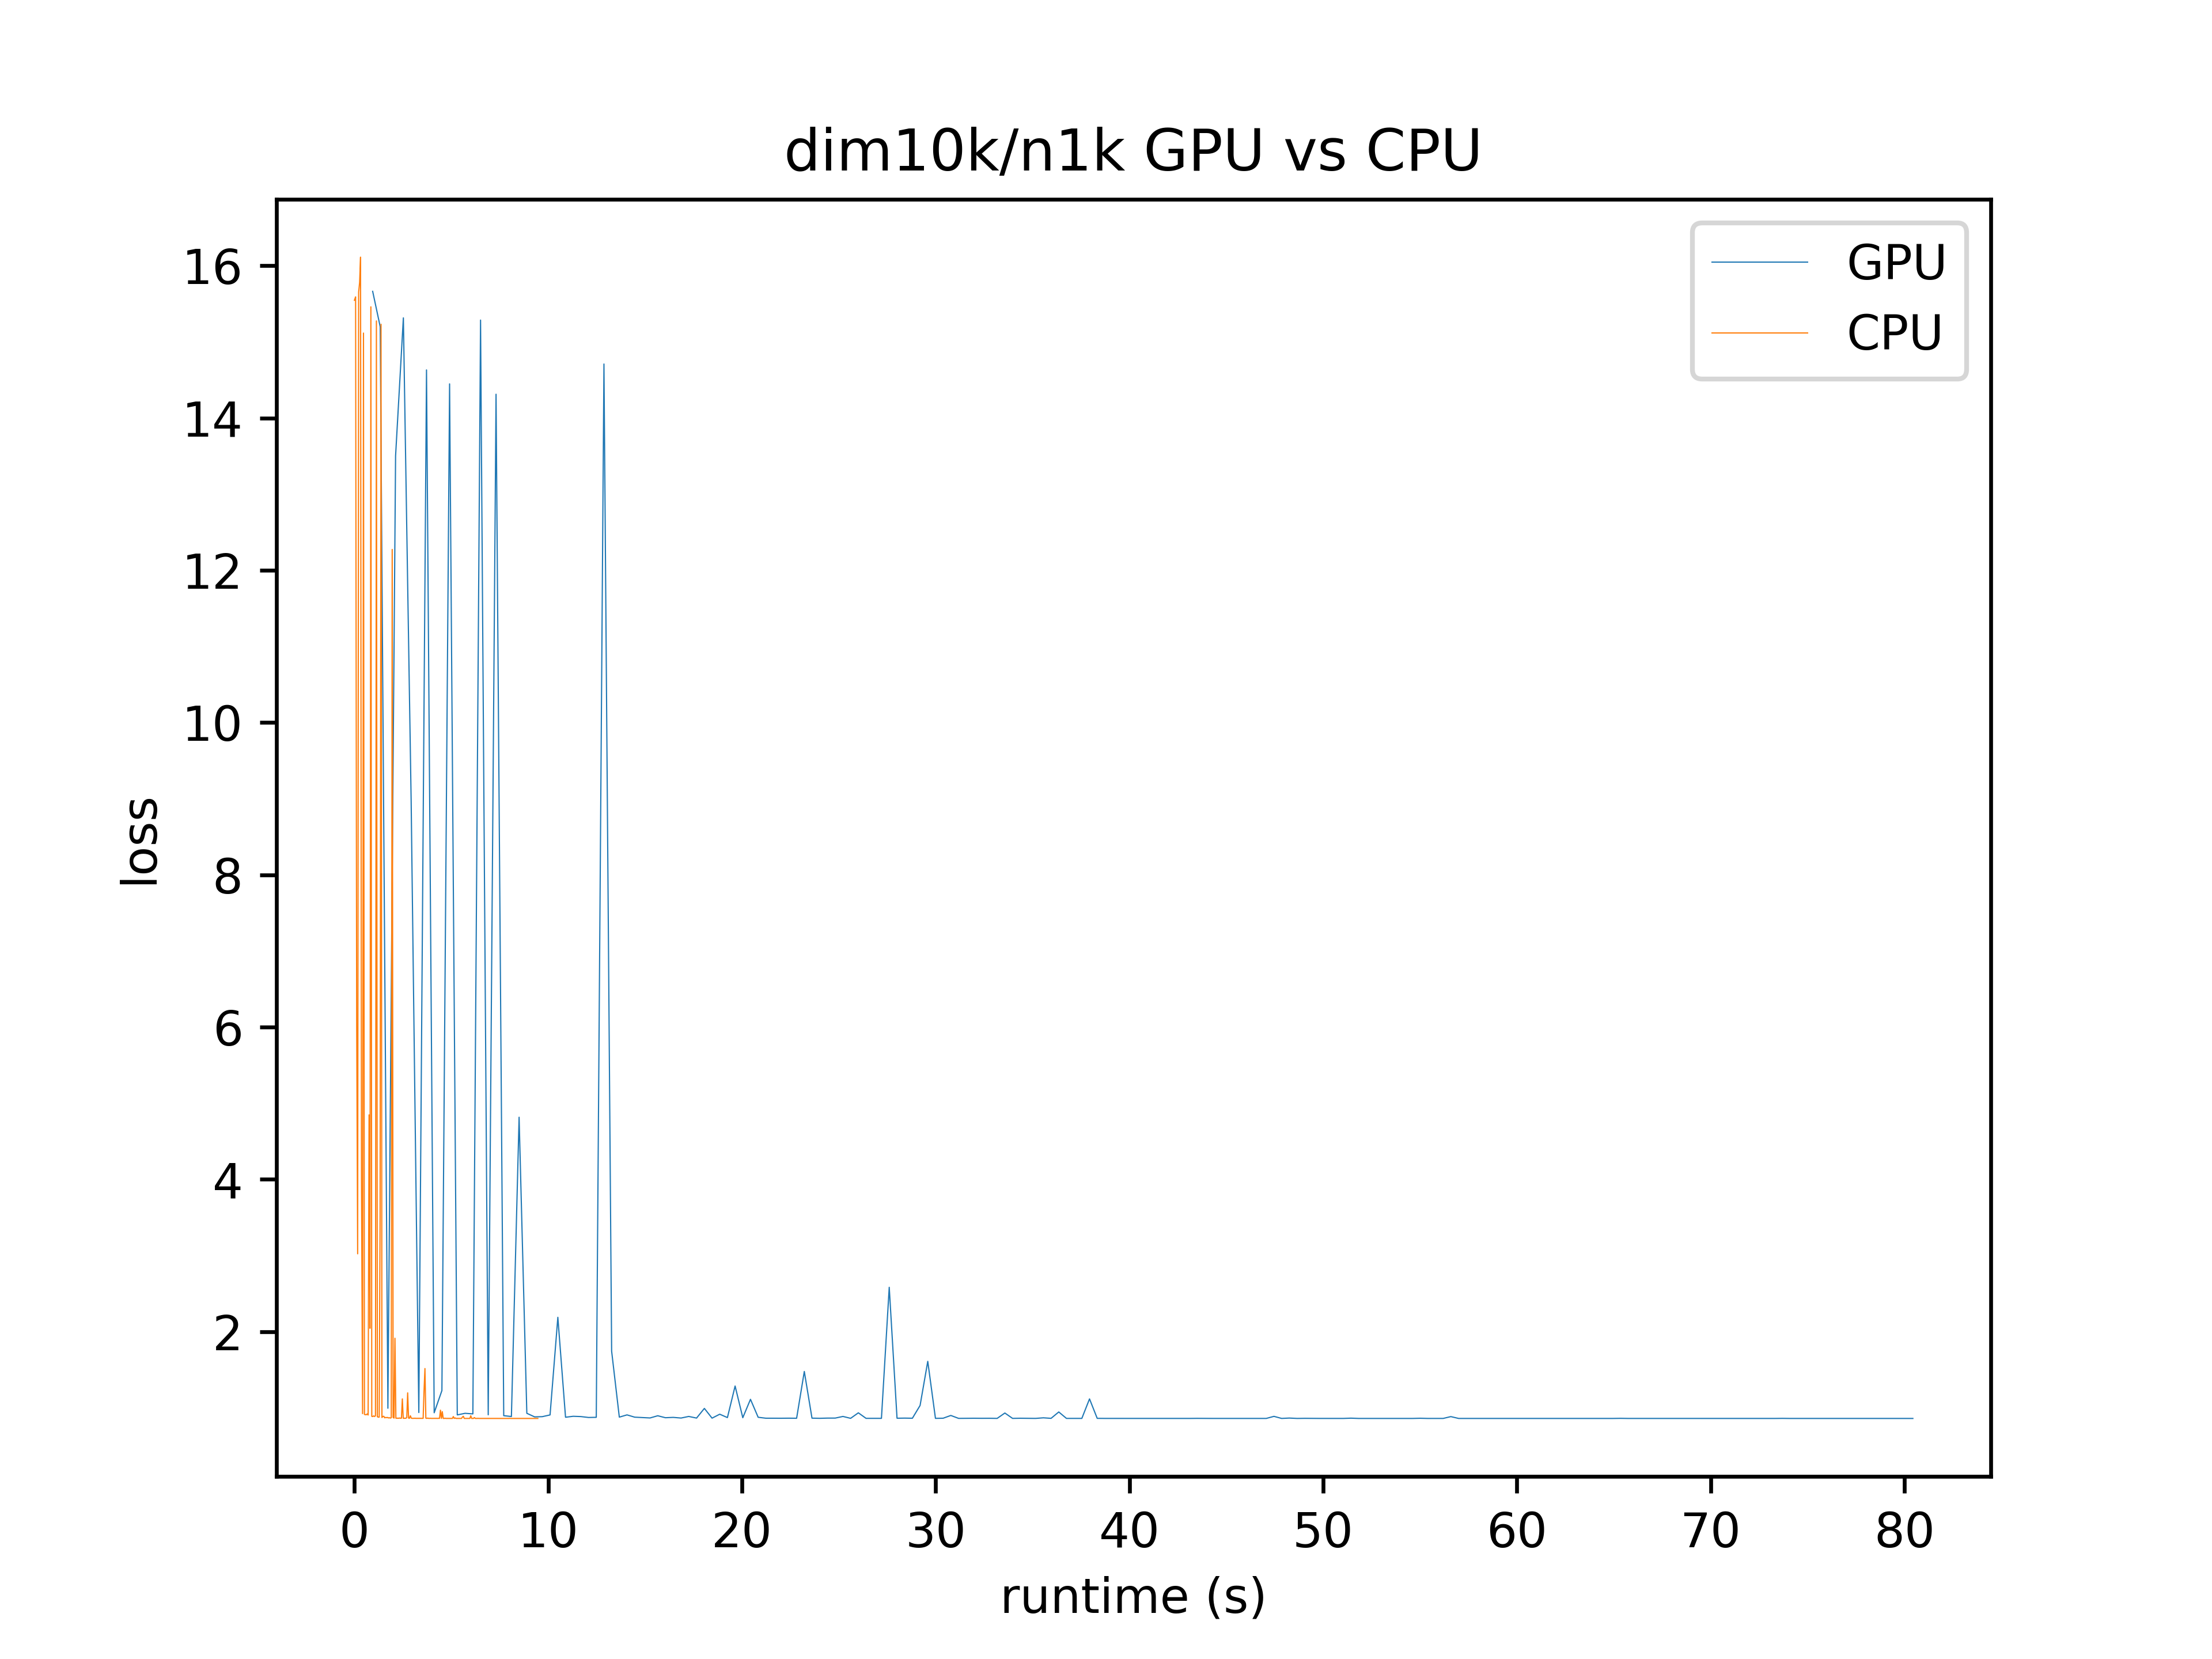
\includegraphics[scale=0.5]{dim10k_CPU_GPU}
\end{figure}
\end{frame}


\begin{frame}{Results - Generated Dataset ($\R^{50k}$, 1000 points)}
  Naive approach\\
  \begin{figure}
    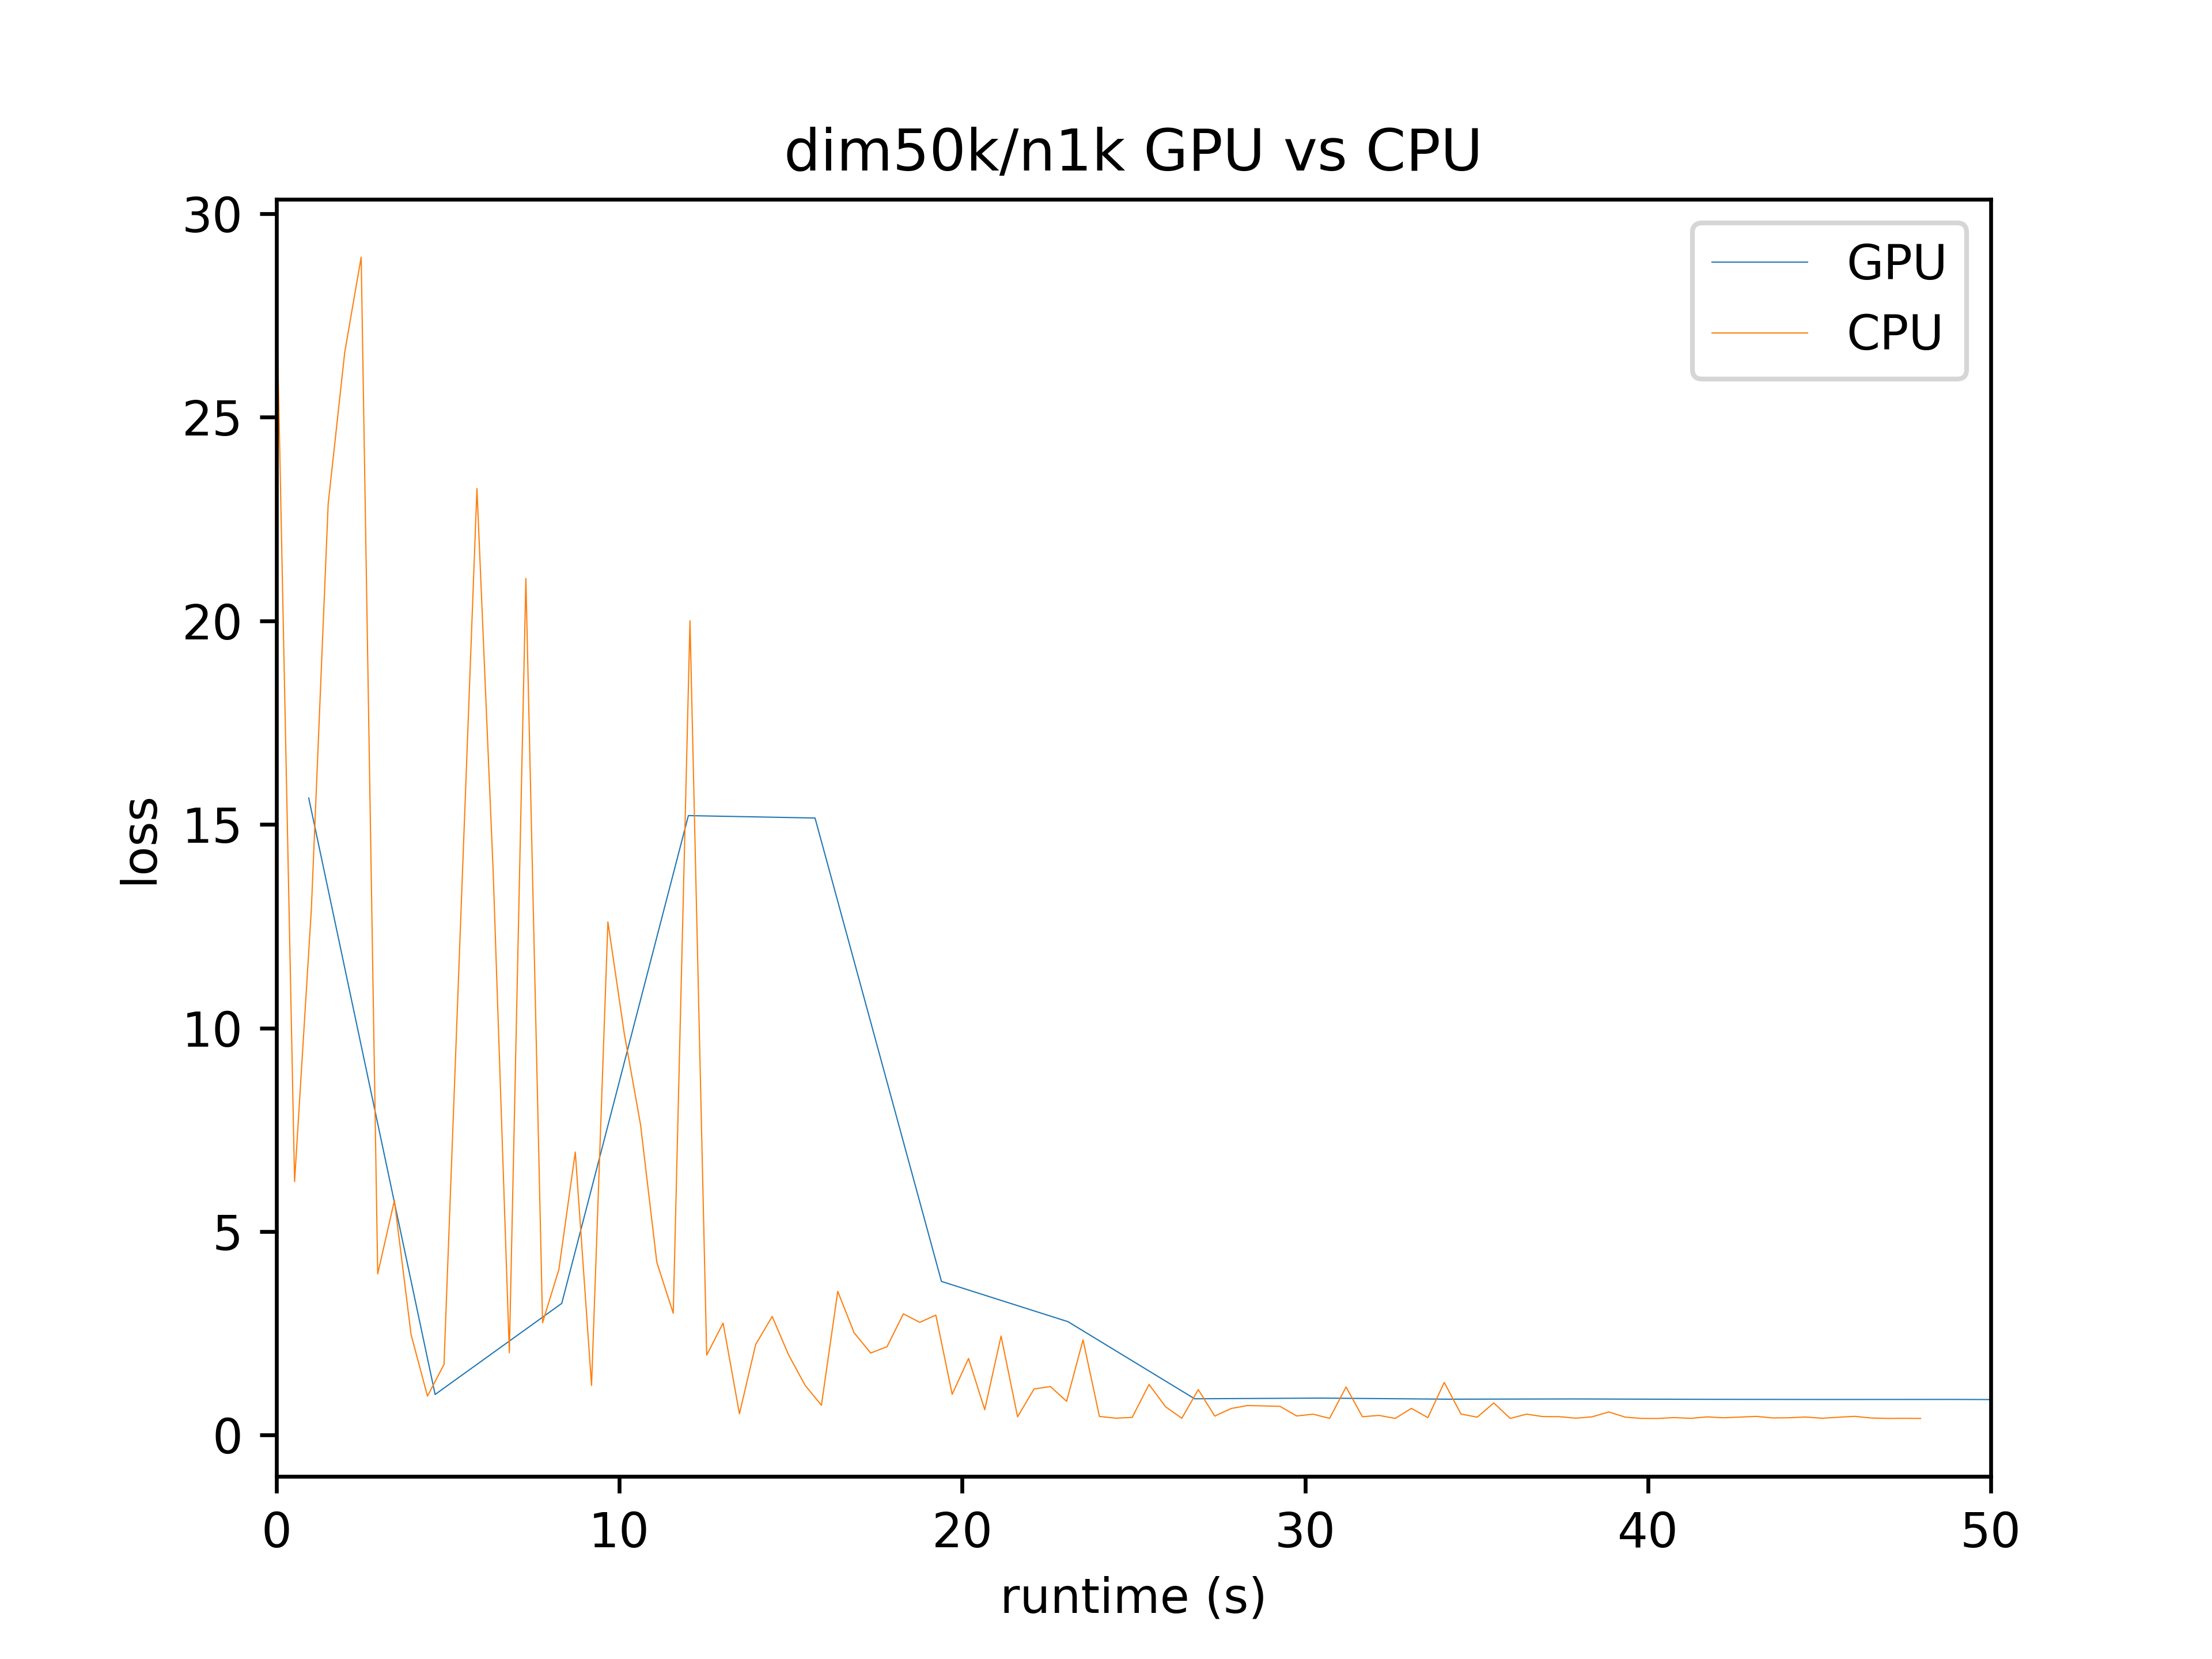
\includegraphics[scale=0.5]{50k_lim}
\end{figure}
\end{frame}


\bibliographystyle{apalike}	
\bibliography{courseProject}

\end{document}


%\AtBeginSection[]
%{
%	\begin{frame}<beamer>
%		\frametitle{Outline for section \thesection}
%		\tableofcontents[currentsection]
%	\end{frame}
%}
%
%\title{Efficient Distributed SDCA}
%
%\begin{document}
%\maketitle
%\begin{frame}{Table of contents}
%\tableofcontents
%\end{frame}
%\section{Overview}


%\end{document}
